\documentclass[fleqn,11pt]{article}

\usepackage[letterpaper,margin=0.75in]{geometry}

\usepackage{amsmath}
\usepackage{booktabs}
\usepackage{graphicx}
\usepackage{listings}

\setlength{\parindent}{1.4em}

\begin{document}

\lstset{
  language=Python,
  basicstyle=\small,          % print whole listing small
  keywordstyle=\bfseries,
  identifierstyle=,           % nothing happens
  commentstyle=,              % white comments
  stringstyle=\ttfamily,      % typewriter type for strings
  showstringspaces=false,     % no special string spaces
  numbers=left,
  numberstyle=\tiny,
  numbersep=5pt,
  frame=tb,
}

\title{Reliable Transport}

\author{Spencer Wood}

\date{February 24, 2017}

\maketitle


I implemented TCP and performed analysis on the relationship between speed and
reliability. The first series of tests were basic transmission tests between the
two nodes. The second involved an implementation of fast retransmit and how
that affected file transfers between the two nodes. The third series of tests
examines the relationship between window size, throughput, and average queueing
delay.\\

All tests were done on a simple 2 node network with a bi-directional link. The
bandwidth of the links was 10Mbps and the propagation delay was 10ms.

\section{Basic Tests}

\subsection{Test \#1}

\indent\indent This test involved transmitting a 10,000 byte text file from the
first node to the second node with a window size of 3,000 bytes and with
various values of packet loss (0\%, 10\%, 20\%, and 50\%).\\

Table \ref{tab:basic_overview_1} shows an overview of the results.

\begin{table}[h]
  \caption{Test \#1 results}
  \label{tab:basic_overview_1}
  \begin{center}
    \begin{tabular}{cccc}
      \toprule
      Packet Loss & Time to Transfer File \\
      \midrule
      0\% & 0.0832s \\
      10\% & 1.1048s \\
      20\% & 3.1056s \\
      50\% & 11.1456s \\
      \bottomrule
    \end{tabular}
  \end{center}
\end{table}

\begin{lstlisting}[caption={Truncated output for 0\% packet loss}]
...
0.0624 n1 (1) sending TCP segment to 2 for 9000
0.0632 n1 (1) handling ACK  8000
0.064 n1 (1) handling ACK  9000
0.0732 n2 (2) received TCP segment from 1 for 9000
0.0732 application got 1000 bytes
0.0732 n2 (2) sending TCP ACK to 1 for 10000
0.0832 n1 (1) handling ACK  10000
File transfer correct!
\end{lstlisting}

\newpage

\begin{lstlisting}[caption={Truncated output for 10\% packet loss}]
...
1.074 n2 (2) sending TCP ACK to 1 for 9000
1.084 n1 (1) handling ACK  9000
1.084 n1 (1) sending TCP segment to 2 for 9000
1.0948 n2 (2) received TCP segment from 1 for 9000
1.0948 application got 1000 bytes
1.0948 n2 (2) sending TCP ACK to 1 for 10000
1.1048 n1 (1) handling ACK  10000
File transfer correct!
\end{lstlisting}

\begin{lstlisting}[caption={Truncated output for 20\% packet loss}]
...
2.0848 n1 (1) sending TCP segment to 2 for 9000
3.0848 n1 (1) sending TCP segment to 2 for 9000
3.0848 n1 (1) retransmission timer fired
3.0956 n2 (2) received TCP segment from 1 for 9000
3.0956 application got 1000 bytes
3.0956 n2 (2) sending TCP ACK to 1 for 10000
3.1056 n1 (1) handling ACK  10000
File transfer correct!
\end{lstlisting}

\begin{lstlisting}[caption={Truncated output for 50\% packet loss}]
...
11.1248 n1 (1) handling ACK  8000
11.1248 n1 (1) sending TCP segment to 2 for 8000
11.1248 n1 (1) sending TCP segment to 2 for 9000
11.1356 n2 (2) received TCP segment from 1 for 8000
11.1356 application got 2000 bytes
11.1356 n2 (2) sending TCP ACK to 1 for 10000
11.1456 n1 (1) handling ACK  10000
File transfer correct!
\end{lstlisting}

\subsection{Test \#2}

\indent\indent This test involved transmitting a 514,520 byte pdf from the
first node to the second node with a window size of 10,000 bytes and with
packet loss of 0\% and 50\%.\\

Table \ref{tab:basic_overview_2} shows an overview of the results.

\begin{table}[h]
  \caption{Test \#2 results}
  \label{tab:basic_overview_2}
  \begin{center}
    \begin{tabular}{cccc}
      \toprule
      Packet Loss & Time to Transfer File \\
      \midrule
      0\% & 1.084416s \\
      50\% & 329.0624s \\
      \bottomrule
    \end{tabular}
  \end{center}
\end{table}

\newpage

\begin{lstlisting}[caption={Truncated output for 0\% packet loss}]
...
1.074416 application got 520 bytes
1.074416 n2 (2) sending TCP ACK to 1 for 514520
1.0816 n1 (1) handling ACK  511000
1.0824 n1 (1) handling ACK  512000
1.0832 n1 (1) handling ACK  513000
1.084 n1 (1) handling ACK  514000
1.084416 n1 (1) handling ACK  514520
File transfer correct!
\end{lstlisting}

\begin{lstlisting}[caption={Truncated output for 50\% packet loss}]
...
328.0416 n1 (1) retransmission timer fired
329.0416 n1 (1) sending TCP segment to 2 for 511000
329.0416 n1 (1) retransmission timer fired
329.0524 n2 (2) received TCP segment from 1 for 511000
329.0524 application got 0 bytes
329.0524 n2 (2) sending TCP ACK to 1 for 514520
329.0624 n1 (1) handling ACK  514520
File transfer correct!
\end{lstlisting}

\section{Fast Retransmit}

\indent\indent I implemented a simple fast transport protocol that resends dropped packets
after 4 duplicate ACKs are received in a row. To measure the impact this has on
file transfer speed, I did two tests, each with a window size of 10,000 bytes
and a loss rate of 20\%. For the first test fast retransmit was turned off and
for the second in t was turned on. In each case the file transfered was a
514,520 byte pdf.\\

Table \ref{tab:fast} shows an overview of the results. Fast retransmit cut down
the transfer time by 90\%.

\begin{table}[h]
  \caption{Test \#2 results}
  \label{tab:fast}
  \begin{center}
    \begin{tabular}{cccc}
      \toprule Fast Retransmit & Packet Loss & Time to Transfer File \\
      \midrule
      No & 20\% & 67.91402s \\
      Yes & 20\% & 6.74282s \\
      \bottomrule
    \end{tabular}
  \end{center}
\end{table}

\begin{lstlisting}[caption={Truncated output for no fast retransmit}]
...
66.8936 n1 (1) handling ACK  514000
67.8936 n1 (1) sending TCP segment to 2 for 514000
67.8936 n1 (1) retransmission timer fired
67.90401600000001 n2 (2) received TCP segment from 1 for 514000
67.90401600000001 application got 520 bytes
67.90401600000001 n2 (2) sending TCP ACK to 1 for 514520
67.91401600000002 n1 (1) handling ACK  514520
File transfer correct!
\end{lstlisting}

\newpage

\begin{lstlisting}[caption={Truncated output for fast retransmit}]
...
6.730415999999962 n2 (2) received TCP segment from 1 for 514000
6.730415999999962 application got 0 bytes
6.730415999999962 n2 (2) sending TCP ACK to 1 for 514520
6.7328159999999615 n2 (2) received TCP segment from 1 for 514000
6.7328159999999615 application got 0 bytes
6.7328159999999615 n2 (2) sending TCP ACK to 1 for 514520
6.742815999999961 n1 (1) handling ACK  514520
File transfer correct!
\end{lstlisting}

\section{Experiments}

\indent\indent The final series of tests examined the relationship between
window size and queueing delay / throughput. Two experiments were performed.\\

The first measured the affect of window size on average packet queueing delay.
The PDF was transferred from the first node to the second node using window
sizes of 1000, 2000, 5000, 10000, 15000, and 20000 bytes. Packet loss was set
to 0\%. The average queueing delay was measured during each run. The results
are shown in figure \ref{fig:queueing}. As window size goes up, queueing delay appears
to increase exponentially. \\

\begin{figure}[!htb]
  \centering
  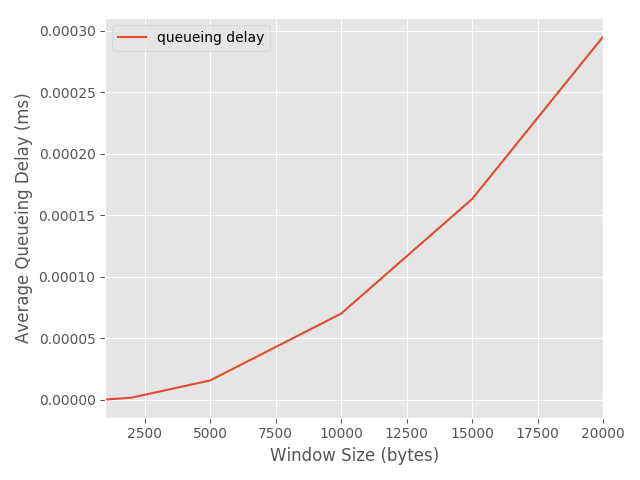
\includegraphics[width=13cm]{queueing.png}
  \caption{Average queueing delay}
  \label{fig:queueing}
\end{figure}

\newpage

The second test measured the affect of window size on throughput. Throughput is
measured as the number of bits transferred over the total number of seconds the
transfer took. The PDF was transferred from the first node to the second node
using window sizes of 1000, 2000, 5000, 10000, 15000, and 20000 bytes. Packet
loss was set to 0\%. The throughput was measured during each run.  The results
are shown in figure \ref{fig:throughput}. As window size increases, throughput appears
to increase linearly.

\begin{figure}[!htb]
  \centering
  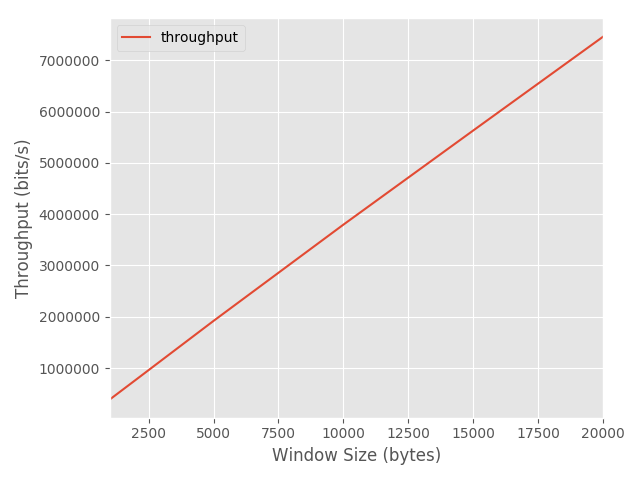
\includegraphics[width=13cm]{throughput.png}
  \caption{Throughput}
  \label{fig:throughput}
\end{figure}

\end{document}
